\documentclass[review]{elsarticle}

\usepackage{lineno,hyperref}
\usepackage{mathtools}
\usepackage{multirow}
\usepackage{adjustbox}
\usepackage{chngpage}
\usepackage{setspace}
\usepackage{amsfonts}
\usepackage[ruled, lined, onelanguage, linesnumbered]{algorithm2e}
\usepackage[usenames,dvipsnames,svgnames,table]{xcolor}
\newcommand{\myfloatalign}{\centering}
\modulolinenumbers[5]

\journal{Applied Soft Computing}

%%%%%%%%%%%%%%%%%%%%%%%
%% Elsevier bibliography styles
%%%%%%%%%%%%%%%%%%%%%%%
%% To change the style, put a % in front of the second line of the current style and
%% remove the % from the second line of the style you would like to use.
%%%%%%%%%%%%%%%%%%%%%%%

%% Numbered
%\bibliographystyle{model1-num-names}

%% Numbered without titles
%\bibliographystyle{model1a-num-names}

%% Harvard
%\bibliographystyle{model2-names.bst}\biboptions{authoryear}

%% Vancouver numbered
%\usepackage{numcompress}\bibliographystyle{model3-num-names}

%% Vancouver name/year
%\usepackage{numcompress}\bibliographystyle{model4-names}\biboptions{authoryear}

%% APA style
%\bibliographystyle{model5-names}\biboptions{authoryear}

%% AMA style
%\usepackage{numcompress}\bibliographystyle{model6-num-names}

%% `Elsevier LaTeX' style
\bibliographystyle{elsarticle-num}
%%%%%%%%%%%%%%%%%%%%%%%
\newtheorem{definition}{Definition}
\begin{document}

\begin{frontmatter}

\title{Enhancing instance-level constrained clustering through differential evolution}

\author[mymainaddress]{Germ\'an Gonz\'alez Almagro\corref{mycorrespondingauthor}}
\cortext[mycorrespondingauthor]{Corresponding author}
\ead{germangalmagro@ugr.es}

\author[mymainaddress]{Salvador Garc\'ia}

\author[mymainaddress]{Another Juan}

\address[mymainaddress]{Department of Computer Science and Artificial Intelligence, University of Granada, 18071 Granada, Spain}

\begin{abstract}
This template helps you to create a properly formatted \LaTeX\ manuscript.
\end{abstract}

\begin{keyword}
\texttt{elsarticle.cls}\sep \LaTeX\sep Elsevier \sep template
\MSC[2010] 00-01\sep  99-00
\end{keyword}

\end{frontmatter}

\linenumbers

\section{Introduction}

\textcolor{red}{Citar a los de las hormigas}\\
\textcolor{red}{Poner un parrafo de aplicaciones del clustering con restricciones}

\section{Background}

%\subsection{Constrained Clustering}

Clustering is the task of grouping instances of a dataset into subsets. The criterion used to assign an instance to a given cluster is the similarity to the rest of elements in that cluster, and the dissimilarity to the rest of instances of the dataset. In this way, the clustering process obtains subsets of instances of the initial data set that present high intra-similarity and low inter-similarity.

In most clustering applications it is common to have some kind of information about the data set to be analyzed. In constrained clustering this information is given in the form of pairs of instances. A constraint states whether the instances which it refers to must, or must not, be assigned to the same cluster. Using this type of information it is possible to obtain a better result than by using completely unsupervised clustering algorithms.

Before formalizing the definition of constraints we must give a notation for the data set. We will note our dataset as $X$, which is a set of $N$ instances with $D$ features. We well refer to the instances of $X$ as $x$. Now, given the definition of dataset, we can distinguish between two types of constraints:

\begin{itemize}

	\item Must-link constraints $c_=(x_j,x_i)$: instances $x_i$ and $x_j$ from $X$ must be placed in the same cluster.

	\item Cannot-link constraints $c_{\neq}(x_i,x_j)$: instances $x_i$ and $x_j$ from $X$ cannot be assigned to the same cluster.

\end{itemize}

The goal of constrained clustering is to find a partition (or clustering) of $K$ clusters $C = {c_1 \cdots c_K}$ of the dataset $X$ that ideally satisfies all constraints in the constraint set. As in the original clustering problem, it must be fulfilled that the sum of instances in each cluster $c_i$ is equal to the number of instances in $X$, which we have defined as $N = |X| = \sum_{i = 1}^{K} |c_i|$.

Knowing how a constraint is defined, Must-link constraints---from now on ML---are an example of an equivalence relation; therefore, ML constraints are reflexive, transitive and symmetric. This way, given constraints $c_=(x_a,x_b)$ and $c_=(x_b,x_c)$ then $c_=(x_a,x_c)$ is verified. In addition, if $x_a \in c_i$ and $x_b \in c_j$ are related by $c_=(x_a,x_b)$, then $c_=(x_c,x_d)$ is verified for any $x_c \in c_i$ and $x_d \in c_j$ \cite{xu2013improving}\cite{davidson2007survey}.

On the other hand, Cannot-link constraints---from now on CL---do not constitute an equivalence relation. However, analogously, given $x_a \in c_i$ and $x_b \in c_j$, and the constraint $c_{\neq}(x_a,x_b)$, then it is also true that $c_{\neq}(x_c,x_d)$ for any $x_c \in c_i$ and $x_d \in c_j$ \cite{davidson2007survey}.

\subsection{The Feasibility Problem}

Given that constrained clustering adds a new element to the clustering problem, we must consider how this element affects the problem complexity. The feasibility problem for non hierarchical constrained clustering was defined by \cite{davidson2005clustering} as in Definition \ref{def1}.

\begin{definition}
	
	\textbf{Feasibility Problem}: given a dataset $X$, a set of constraints $R$, and the bounds on the number of clusters $K_l \leq k \leq K_u$. Does there exists a partition $C$ of $X$ with $k$ clusters such that all constraints in $R$ are satisfied? \cite{davidson2007survey}\cite{davidson2005clustering}
	\label{def1}
	
\end{definition}

In \cite{davidson2005clustering} it is proven that, when $K_l = 1$ and $K_u \ge 3$, the feasibility problem for constrained clustering is $\mathbf{NP}$-complete, by reducing it from the Graph K-Colorability problem. (It is also proven that it is not harder than it, so both have the same complexity.) Table \ref{tab:feasibility} shows feasibility problem complexity for different types of constraints.

\begin{table}[!h]
	\centering
	%\setlength{\arrayrulewidth}{1mm}
	\setlength{\tabcolsep}{7pt}
	\renewcommand{\arraystretch}{1.2}
	%\resizebox{\textwidth}{!}{
		\begin{tabular}{c c}
			\hline
			Constraints & Complexity \\
			\hline
			Must-Link & $\mathbf{P}$\\
			Cannot-Link & $\mathbf{NP}$-complete\\
			ML and CL & $\mathbf{NP}$-complete\\
			\hline
			
		\end{tabular}%}
	\caption{Feasibility problem complexity \cite{davidson2005clustering}}
	\label{tab:feasibility}
\end{table}

These complexity results show that feasibility problem with CL constraints is intractable and hence constrained clustering is intractable too. For more details on constrained clustering complexity see \cite{davidson2005clustering}.

\textcolor{red}{El parrafo de abajo esta bien?}

Intractable problems are hard to solve with deterministic and exact methods. That is the reason why applying heuristics-guided and population-based algorithms constitute a good approach to find quality solutions to the constrained clustering problem.

\subsection{Short insertion to Differential Evolution}

To introduce Differential Evolution--from now on DE--we take as basis the review of the state-of-the-art performed by \cite{das2011differential}, where you can find a very detailed analysis on DE an its variants.

The first article written on differential evolution emerged in 1995 as a technical report written by \cite{noman2008differential}. From that moment on, DE's reputation was manifested in congresses and competitions where it was able to obtain competitive results that rivaled the state of the art of that moment. Specifically DE excelled in real optimization problems.

DE arises as a variant of population-based evolutionary algorithms, its goal is to perform an intelligent search in the problem's solutions space in the most optimized and effective possible way.

Like most evolutionary algorithms, DE uses a population of individuals $P$, where each individual $p_i$ is a vector of real values $p_i = \{p_{i,1},\cdots,p_{i,D}\}$ that serve as parameters for the function to be optimized. These individuals are considered solutions to the problem.

To guide the optimization process, we use an objective function. DE's task is to seek the parameter vector $p_i$ that minimizes a function such that $f(p_i)(f: \Omega \subseteq \mathfrak{R}^D \rightarrow \mathfrak{R})$, where $f(p_i^*) < f(p_i)$ for all $p_i \Omega$ with omega a nonempty finite set that is the search domain.

\begin{figure}[!h]
	\centering
	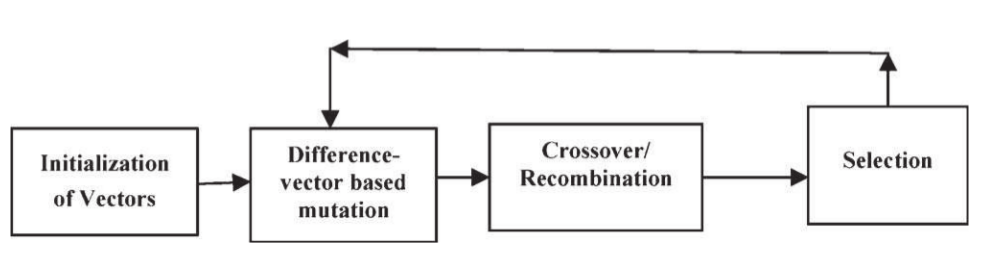
\includegraphics[scale=0.4]{Figures/DEop.png}
	\caption{DE optimization process \cite{das2011differential}.}\label{img:DE}
\end{figure}

DE optimization process works through a simple cycle of stages, presented in Figure \ref{img:DE} that we can summarize stages in as follow:

\begin{itemize}
	
	\item \textbf{Initialization of Vectors}: DE begins with a randomly initiated populations of $N$ $D$-dimensionals arrays of parameters. These vectors constitute a candidate solution for the problem to solve.
	
	\item \textbf{Difference-vector based mutation}: DE introduces diversity on the population via mutation operator. This operator is applied to each individual of the population, known ins this context as parent vector. It combines the parent vector with two randomly selected vectors from the population by applying an arithmetic operator to them. The result of this process is a mutant vector.
	
	\item \textbf{Crossover/Recombination}: The mutant vector exanges some components with its associated parent to from a trial vector, which will be the candidate to replace the parent vector. There exist several strategies to generate this trial vector, we will not delve into them but they can be found in \cite{das2011differential}.
	
	\item \textbf{Selection}: The newly generated trial vector is compared with its associated parent using the objective function. If the trial vector is better than the parent, then it will replace the parent in the next generation. It is worth noting that, following this strategy, the population never degenerates, only get better or remains the same.
	
\end{itemize}

Even though DE was a major breakthrough in terms of real optimization, many variants have been developed since its invention that provide better results. We will focus on the SHADE variant, which adaptively optimizes some of the DE parameters (see Section \ref{sec:SHADE}).


\section{Brief Review of the BRKGA Algorithm}

The biased random-key genetic algorithm---from now on BRKGA---was first proposed by \cite{gonccalves2011biased} as a generalization of the random-key genetic algorithm \cite{bean1994genetic}.

In BRKGA, each solution---also called individual---is represented as a vector of values within the interval $[0,1]$. However, this vector is not a solution to the problem but a representation of it. This allows us to abstract the details of the problem in order to apply a genetic algorithm that operates with real coding. Therefore, a deterministic decoder is necessary to obtain the actual solution to the problem from the vector that encodes it.

BRKGA also requires a fitness function to evaluate each individual. This function takes the decoded solution as input and provides its fitness value as output. It is designed specifically for each problem.

The BRKGA optimization process is completely independent of the problem to solve. First, a population $P$ of $p_{size}$ vectors of random-keys is initialized, and this will be the initial generation. Each random-key vector $p_i$ has $N$ random-keys in it. The population is sorted by the fitness value $f_i$ of each $p_i$ to select the first $p_e$ individuals, this is, the elite of the population. The elite will be preserved in the next generation without modification. To introduce diversity, a number $p_m$ of new random-keys vectors are also included in the next generation. The remaining individuals of the new generation ($p_{size} - p_e - p_m$) are obtained through crossovers between elite and non-elite parents \cite{de2017comparison}.

\subsection{Adaptation of BRKGA for Constrained Clustering} \label{sec:AdaptationofBRKGA}

An adaptation of BRKGA for constrained clustering was proposed in \cite{de2017comparison}.

Their method randomly initializes a population of random-key vectors, each one with $N$ random-keys. The decoder divides the interval $[0,1]$ in $K$ intervals, so there exists a correspondence between each random-key and the integer corresponding to the interval which it lies in. Table \ref{tab:decodingrk} shows an example of random-key decoding for $K = 3$. Note that extreme values 0 and 1 can also appear in a random-key vector.

\begin{table}[!h]
	\centering
	%\setlength{\arrayrulewidth}{1mm}
	\setlength{\tabcolsep}{7pt}
	\renewcommand{\arraystretch}{1.2}
	\resizebox{\textwidth}{!}{
	\begin{tabular}{|c|c|c|c|c|c|c|c|c|c|c|}
		\hline
		Index & 1 & 2 & 3 & 4 & 5 & 6 & 7 & 8 & 9 & 10 \\
		\hline
		Random-key & 0.12 & 0.37 & 0.66 & 0.56 & 0.00 & 0.97 & 0.23 & 0.25 & 0.15 & 1.00 \\
		\hline
		Clusters & 1 & 2 & 2 & 2 & 1 & 3 & 1 & 3 & 1 & 3 \\
		\hline

	\end{tabular}}
	\caption{Random-key decodification example \cite{de2017comparison}}
	\label{tab:decodingrk}
\end{table}

Once the decoded solution has been obtained, the fitness value of the solution is computed as in Equation \eqref{eq1}.

\begin{equation}
f_i = z_i + \overbrace{(\mu * N * {infeasibility}_i)}^{penalty}
\label{eq1}
\end{equation}

Where $\mu$ is a high value, $infeasibility_i$ is the number of non-satisfied constraints and $z_i$ is the within-cluster-sum-of-squares which can be computed as in Equation \eqref{eq2}.

\begin{equation}
z_i = \sum_{c_j \in C_i} \left[ \frac{\sum_{x_a, x_b \in c_j} d_D^2(x_a,x_b)}{|c_j|}\right]
\label{eq2}
\end{equation}

Where $C_i$ is the partition of dataset $X$ defined by solution $p_i$, and $(x_a, x_b)$ are instances in the cluster $c_j$ such that $a \neq b$ and the distance between each pair of instances in $c_i$ is included in the sum only once.

In \cite{de2017comparison} authors also added a new element to BRKGA, a local search procedure. This local optimization method is applied to each decoded individual in each generation, but its results are not transferred to the individual, so that diversity is maintained. Thus, the individuals produced by the local search are only used to update the best solution found so far if needed. For more details on BRKGA see \cite{de2017comparison}.

\section{The SHADE Optimization Method} \label{sec:SHADE}

Success history based adaptive differential evolution---from now on SHADE---is an optimization method based on differential evolution. Proposed by \cite{tanabe2013success}, it was an improvement for the JADE model, created by \cite{zhang2009jade}.

Unlike JADE, which only considers the parameters used in the previous generation, SHADE uses a historical record of successful parameters as a mechanism for adapting parameters involved in the process of creating new generations.

\subsection{SHADE Operators}

As in differential evolution, SHADE employs mutant generation, crossover and replacement operators to explore the space of solutions and bring in new generations of individuals.

The mutation strategy used by SHADE is known as current-to-$p$best/1, and the expression that generates new individuals is described in Equation \eqref{eq3}.

\begin{equation}
m_{[i,G]} = p_{[i,G]} + F_i * (p_{[pbest, G]} - p_{[i,G]}) + F_i * (p_{[r1, G]} - p_{[r2,G]})
\label{eq3}
\end{equation}

Where $m_{[i,G]}$ is the mutant vector, which is generated with an individual $p_{[i,G]}$ from the population [serving as a starting point]. Indices $r1$ and $r2$ are random values in the range $[0,N]$, different from $i$ and from each other. The individual $p_{[pbest, G]}$ is randomly selected from among the best $N \times pbest\;|\;pbest\in [0,1]$ individuals in the population. This way, the parameter $p$ controls the greediness of the mutation strategy. The parameter $F_i$ defines the magnitude of the operator.

After generating the mutant vector $m_{[i,G]}$, it is combined with the parent $p_{[i,G]}$ vector by means of a crossover operator; the result is the trial vector. SHADE uses the Binomial crossover operator, which is defined by the Equation \eqref{eq4}.

\begin{equation}
t_{[j,i,G]} = \left\{ \begin{array}{lc}
m_{[j,i,G]} &   if \;\; \text{rand}[0,1) \le CR_i \;\; or \;\;j = j_{rand} \\
p_{[j,i,G]} &  \text{otherwise}
\end{array}
\right.
\label{eq4}
\end{equation}

Where $rand[0,1)$ is a random number selected from a normal distribution in the range $[0,1)$, $j_{rand}$ is a random integer selected from the range $[1,D]$, and $CR \in [0,1]$ is the crossover ratio.

The SHADE replacement operator determines the survivors individuals for the next generation. It compares each parent $x_{[i,G]}$ with the trial vector $_{[j,i,G]}$, generated based on it. The best one of these two individuals will survive for the next generation. Equation \eqref{eq5} shows this concept.

\begin{equation}
p_{[i,G + 1]} = \left\{ \begin{array}{lc}
t_{[i,G]} &   if \;\; f(t_{[i,G]}) \le f(p_{[i,G]}) \\
p_{[i,G]} &  \text{otherwise}
\end{array}
\right.
\label{eq5}
\end{equation}

To maintain diversity, SHADE can make use of an external archive $A$, in which parents $p_{[i,G]}$ who were replaced by their associated trial vector $t_{[i,G]}$ are saved. To make use of the archive, we will consider that the individual $p_{[r2,G]}$ from Equation \eqref{eq3} is selected from $P \cup A$. The archive size is the same as the population size. When the size of $A$ exceeds the size of $P$, random individuals are selected for removal to make room for new ones.

The parameters $p$, $F_i$ and $CR_i$ are difficult to adjust and their selection is not trivial, as they largely determine the success of the optimization process. These are the parameters that SHADE adaptively optimizes using the mentioned history record.

\subsection{SHADE Parameter Adaptation Method}

The SHADE method stores in memory a structure with $H$ entries for parameters $F_i$ and $CR_i$, as shown in Table \ref{tab:SHADEmemory}. This structure is initialized with the value $0.5$ for all entries.

\begin{table}[!h]
	\centering
	%\setlength{\arrayrulewidth}{1mm}
	\setlength{\tabcolsep}{13pt}
	%\renewcommand{\arraystretch}{0.9}
	\resizebox{\textwidth}{!}{
	\begin{tabular}{|c|c|c|c|c|c|}
		\hline
		 Index & 1 & 2 & $\cdots$ & $H - 1$ & $H$ \\
		 \hline
		 \hline
		 $M_{CR}$ & $M_{[CR,1]}$ & $M_{[CR,1]}$ & $\cdots$ & $M_{[CR,H-1]}$ & $M_{[CR,H]}$ \\
		 \hline
		 $M_{F}$ & $M_{[F,1]}$ & $M_{[F,1]}$ & $\cdots$ & $M_{[F,H-1]}$ & $M_{[F,H]}$ \\
		\hline

	\end{tabular}}
	\caption{Historical memory $M_{CR}$, $M_{F}$ used by SHADE \cite{tanabe2013success}}
	\label{tab:SHADEmemory}
\end{table}

In each generation, parameters $CR_i$ and $F_i$ are calculated on the basis of the existing history by applying Equations \eqref{eq6} and \eqref{eq7}:

\begin{equation}
CR_i = \text{randn}_i(M_{[CR,r_i]}, 0.1)
\label{eq6}
\end{equation}

\begin{equation}
F_i = \text{randc}_i(M_{[F,r_i]}, 0.1)
\label{eq7}
\end{equation}

where $randn(\mu, \sigma^2)$ and $randc(\mu, \sigma^2)$ are random values from normal and Cauchy distributions respectively, with mean $\mu$ and variance $\sigma^2$. When a value for $CR_i$ outside of the range $[0,1]$ is generated, it is replaced by the corresponding limit value. If $F_i > 1$, then it is truncated to $1$; conversely, if $F_i < 0$, then Equation \eqref{eq7} is applied as many times as needed to obtain a legal value.

SHADE keeps two auxiliar sets $S_{CR}$ and $S_F$ to store the $CR_i$ and $F_i$ values that were successfully used to generate a trial vector that replaced the parent. At the end of each generation, the content of the memory $M$ is updated following Equations \eqref{eq8} and \eqref{eq9}.

\begin{equation}
M_{[CR,h,G+1]} = \left\{ \begin{array}{lc}
\text{mean}_{WA} (S_{CR}) &   if \;\; S_{CR} \neq \emptyset \\
M_{[CR,h,G+1]} &  otherwise
\end{array}
\right.
\label{eq8}
\end{equation}

\begin{equation}
M_{[F,h,G+1]} = \left\{ \begin{array}{lc}
\text{mean}_{WL} (S_{F}) &   if \;\; S_{F} \neq \emptyset \\
M_{[F,h,G+1]} &  otherwise
\end{array}
\right.
\label{eq9}
\end{equation}

The $h \;\; (0 \le h \le H)$ index specifies the position of the memory $M$ to be updated. This index is initialized to $0$ at the beginning of the optimization process and increased by one after each generation. When $h \ge H$ then $h$ is reset to 1. It is worth noting that, when there is a generation with no trial vectors successfully replacing their parents, no update of $M$ is done.

In Equation \ref{eq8}, the term $mean_{WA} (S_{CR})$ is the weighted mean, which is computed following Equations \eqref{eq10} and \eqref{eq11}, proposed by \cite{peng2009multi} to prevent $CR$ from converging to small values.

\begin{equation}
\text{mean}_{WA} (S_{CR}) = \sum_{i = 1}^{|S_{RC}|} \omega_i * S_{[RC,i]}
\label{eq10}
\end{equation}

\begin{equation}
\omega_i = \frac{\Delta f_i}{\sum_{i = 1}^{|S_{RC}|} \Delta f_i}
\label{eq11}
\end{equation}

where $\Delta f_i = |f(t_{[i,G]}) - f(p_{[i, G]})|$, which is the amount of improvement obtained from the trial vector with respect to the parent.

In Equation \ref{eq9} the term $mean_{WL} (S_{F})$ refers to the weighted Lehmer mean, which is computed as in Equation \eqref{eq12} (proposed by \cite{tanabe2013success}).

\begin{equation}
\text{mean}_{WL} (S_{F}) = \frac{\sum_{i = 1}^{|S_{F}|} \omega_i * S^2_{[F,i]}}{\sum_{i = 1}^{|S_{F}|} \omega_i * S_{[F,i]}}
\label{eq12}
\end{equation}

Unlike parameters $S_{CR}$ and $S_F$, the parameter $pbest$ from Equation \eqref{eq3}, used to set the greediness of the mutation strategy, is not included in the adaptive optimization process. However, it is not static: it is calculated for each individual $p_i$ of the population following Equation \eqref{eq13}.

\begin{equation}
pbest_i = \text{randn}[2/N, 0.2]
\label{eq13}
\end{equation}

such that there is always at least two individuals to choose between.

\subsection{Adaptation of SHADE for constrained clustering}

For the adaptation of SHADE to the problem of constrained clustering, we will take some of the elements that allowed us to adapt it to BRKGA. To begin with, we will use random-keys to create the individuals of the population; this way, each individual is defined as a vector of random-keys. Additionally, we will also reuse the same initialization method and the same decoder used in BRKGA (see Section \ref{sec:AdaptationofBRKGA}).

However, we propose a new fitness function to evaluate the quality of the individuals of the population, Equation \eqref{eq14}, whose element $z_i$ is obtained as in Equation \eqref{eq2}.

\begin{equation}
f_i = z_i * (infeasibility + 1)
\label{eq14}
\end{equation}

Note that in Equation \eqref{eq14} no parameter is involved that cannot be calculated from the dataset or constraints, whereas in Equation \eqref{eq1} the $\mu$ parameter must be calculated and optimized for each individual problem.

We found that with the fitness function defined in \eqref{eq1} there is no competition between the penalty term and the within-cluster-sum-of-squares term, because the penalty is always significantly larger than it or zero. This can bias the exploration of the solution space, restricting it in practice to those that satisfy all the constraints, even if the within-cluster-sum-of-squares is still improvable by moving two instances involved in a constraint to different clusters without violating that constraint.

With Equation \eqref{eq14} we try to find a trade-off between the within-cluster-sum-of-squares and the penalty term, allowing solutions that violate a certain number of constraints to compete with those who violate a smaller number of them but score a better within-cluster-sum-of-squares.

To put those concepts clear we consider a toy dataset and three partitions over it. Dataset from Figure \ref{img:toydatasets} contains 100 instances and a single ML constraint between two instances from the same class. Partitions $C_0$ and $C_1$ do not violate the constraint ($infeasibility = 0$), while $C_2$ does violate it ($infeasibility = 1$). 

\begin{figure}[bth]
	\myfloatalign
	{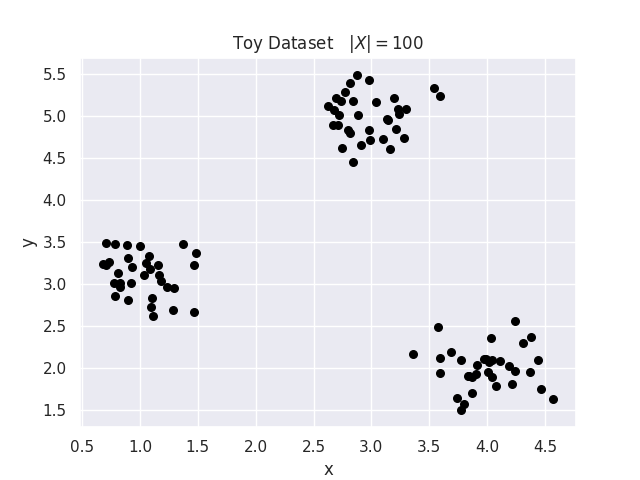
\includegraphics[width=.45\linewidth]{Figures/Dataset}} \quad
	%\subfloat[Imagen original]
	{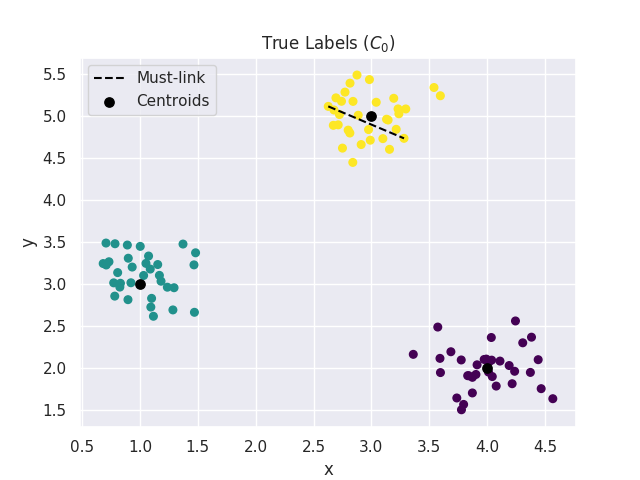
\includegraphics[width=.45\linewidth]{Figures/C0}} \quad
	%\subfloat[Clustering sin restricciones]
	{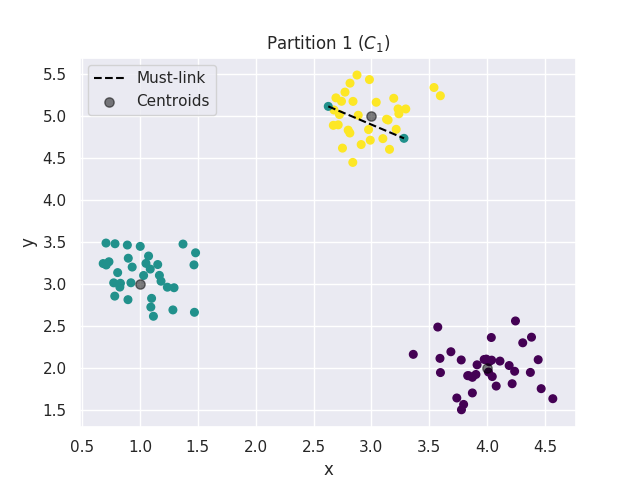
\includegraphics[width=.45\linewidth]{Figures/C1}} \quad
	%\subfloat[Clustering con restricciones]
	{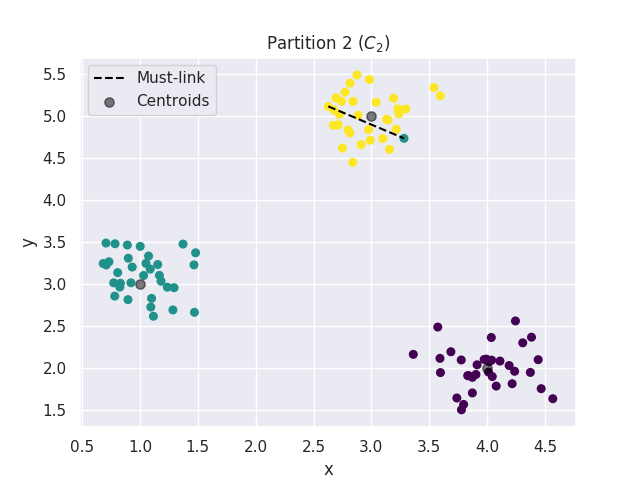
\includegraphics[width=.45\linewidth]{Figures/C2}} \quad
	\caption{Three partitions over a toy dataset.}
	\label{img:toydatasets}
\end{figure}

Table\ref{tab:fitnessfunctions} shows fitness functions values for each partition from Figure \ref{img:toydatasets}. We call $f_1$ to the function presented in Equation \eqref{eq1} and $f_2$ to the function presented in Equation \eqref{eq14}.

\begin{table}[!h]
	\centering
	\setlength{\tabcolsep}{7pt}
	\renewcommand{\arraystretch}{1.3}
	%\begin{adjustwidth}{-1in}{-1in}
	\resizebox{\textwidth}{!}{
		\begin{tabular}{c c c c c c}
			\hline
			\multirow{2}{*}{Partition} &
			\multicolumn{2}{c}{Expression} &&
			\multicolumn{2}{c}{Value} \\
			\cline{2-3} \cline{5-6}
			& $f_1$ & $f_2$ && $f_1$ & $f_2$ \\
			\hline
			$C_0$ & $z_0$ & $z_0$ && $0.457$  & $0.457$  \\
			$C_1$ & $z_1$ & $z_1$  && $0.540$  & $0.540$  \\
			$C_2$ & $z_2 + (\mu * N * infs)$ & $z_2 * (infs + 1)$  && $0.503 + 1000 = 1000.503$ &  $0.503 * 2 = 1.005$ \\
			\hline
			
		\end{tabular}}
		%\end{adjustwidth}
		
	\caption{Expression and value of fitness functions over three partitions. ($\mu = 10$)}
	\label{tab:fitnessfunctions}
\end{table}

Results in Table \ref{tab:fitnessfunctions} are a clear example of the above. In the general case, with $f_2$ the penalty for violating constraints is proportional to the within-cluster-sum-of-squares, the lower it is the lower the penalty. This is not the case with $f_1$, whose penalty term is independent of the within-cluster-sum-of-squares, which can result in a difference of several orders of magnitude between partitions satisfying different number of constraints.

As in \cite{de2017comparison} we apply a local optimization procedure to the individuals of the population, without transferring its results to the individual to maintain diversity. The difference is that we do not apply it to the whole population but only to a number $p_e$ of individuals considered as the elite of the population. The percentage of individuals considered as elite must be determined for each case.

Algorithms \ref{alg:SHADE} shows overall SHADE optimization process and is an adaptation of the one that can be found on \cite{tanabe2013success} to include the local search procedure presented in Algorithm \ref{alg:LS}.

\begin{algorithm}
	\SetNlSty{textbf}{[}{]}
	\SetNlSkip{0.5em}
	\setstretch{1.2}
	\SetKwFunction{Sort}{Sort}
	\SetKwFunction{LocalSearch}{LocalSearch}
	\KwIn{Dataset $X$, constraints sets $c_=$ and $c_{\neq}$, population size $p_{size}$, elite size $p_e$, number of clusters $K$.}
	\tcp{Initialization phase}
	$G \leftarrow 0$\\
	Initialize population $P_0 \leftarrow \{p_{[1,0]}, \cdots, p_{[p_{size},0]}\}$\\
	Initialize all values in $M_{CR}$, $M_F$ to 0.5\\
	$A \leftarrow \emptyset$; $h \leftarrow 1$\\
	\tcp{Main loop}
	\While{Termination criteria are not met}{
		
		$S_{CR} \leftarrow S_F \leftarrow \emptyset$\\
		$P_G \leftarrow$ \Sort{$P_G$} \tcp{Sort the population}
		\tcp{Apply a LS procedure to the elite of the population}
		\LocalSearch{$\{p_{[1,G]}, \cdots, p_{[p_{e},G]}\}$}\\
		\For{$i \in [1,p_{size}]$}{
			$r_i \leftarrow$ randInt$[1,H]$\\
			$CR_{[i,G]} \leftarrow$ randn$_i(M_{[CR,r_i]}, 0.1)$\\
			$F_{[i,G]} \leftarrow$ randc$_i(M_{[F,r_i]}, 0.1)$\\
			$p_{[i,G]} \leftarrow$ rand$[N/2, 0.2]$\\
			Generate trial vector $t_{[i,G]}$ by current-to-$p$best/1/bin\\
			
			\eIf{$f(t_{[i,G]}) \le f(p_{[i,G]})$}{
				$p_{[i,G + 1]} \leftarrow t_{[i,G]}$
			}{
				$p_{[i,G + 1]} \leftarrow p_{[i,G]}$
			}
			
			\If{$f(t_{[i,G]}) < f(p_{[i,G]})$}{
				$p_{[i,G]} \rightarrow A$;
				$CR_{[i,G]} \rightarrow S_{CR}$;
				$F_{[i,G]} \rightarrow S_{F}$
			}
			
		}
		Whenever $|A| > |P|$, randomly select an individual from $A$ to be deleted so that $|A| \le |P|$\\
		\If{$S_{CR} \neq \emptyset$ \textbf{and} $S_{F} \neq \emptyset$}{
			Update $M_{[CR,h]}$ and $M_{[F,h]}$ based on $S_{CR}$ and $S_{F}$\\
			$h \leftarrow (h + 1) \mod H$
		}
		$G++$
	}
	\caption{Modified SHADE}\label{alg:SHADE}
\end{algorithm}

\begin{algorithm}
	\SetNlSty{textbf}{[}{]}
	\SetNlSkip{0.5em}
	\setstretch{1.2}
	\SetKwFunction{RandomShuffle}{RandomShuffle}
	\SetKwRepeat{Do}{do}{while}
	\KwIn{Dataset $X$, constraints sets $c_=$ and $c_{\neq}$, decoded random-key vector (solution) $S$, number of clusters $K$.}
	\BlankLine
	\While{$improvement$}{
		$improvement \leftarrow$ \texttt{false} \\

		$s_i \leftarrow $ Select random object from $S$\\
		\tcp{Random shuffle labels set}
		$RSL \leftarrow $ \RandomShuffle{$\{1,\cdots,K\}$}\\
		\For{$c \in RSL$}{
			$S^\prime \leftarrow S$\\
			$S^\prime$\texttt{[}$s_i$\texttt{]} $\leftarrow c$ \tcp{Move object $s_i$ to cluster $c$}
			
			\If{$f(S^\prime) < f(S)$}{
				$S \leftarrow S^\prime$\\
				$improvement \leftarrow$ \texttt{true} \\
			}
		}	
	}
	\BlankLine
	\KwRet ($S$)
	
\caption{Local Search}\label{alg:LS}
\end{algorithm}

\clearpage

\section{Experimental Setup}

For our experiments we will compare the results obtained by BRKGA and SHADE over XX datasets. Most of the datasets used can be found at the \href{https://sci2s.ugr.es/keel/category.php?cat=clas}{Keel-dataset repository}\cite{triguero2017keel}, though some of them have been obtained via
\href{https://scikit-learn.org/stable/datasets/index.html}{\texttt{scikit-learn} python package} \cite{scikit-learn}. Table \ref{tab:datasets} present a summary the main features of all datasets used. \textcolor{red}{Esta bien citar tambien al sklearn? Que paper de keel cito, 2017 o 2011?}

\begin{table}[!h]
	\centering
	%\setlength{\arrayrulewidth}{1mm}
	%\setlength{\tabcolsep}{5pt}
	%\renewcommand{\arraystretch}{1.2}
	%\resizebox{\textwidth}{!}{
	\small
	\begin{tabular}{l c c c}
		\hline
		Name & No. Instances & No. Classes & Features \\
		\hline
		Appendicitis & 106 & 2 &  \\
		Balance & 625 & 3 &  \\
		Boston & 506 & 229 &  \\
		Breast Cancer & 569 & 2 &  \\
		Bupa & 345 & 2 &  \\
		Circles & 300 & 2 &  \\
		Contraceptive & 1473 & 3 &  \\
		Diabetes & 442 & 214 &  \\
		Ecoli & 336 & 8 &  \\
		Glass & 214 & 6 &  \\
		Haberman & 306 & 2 &  \\
		Hayesroth & 160 & 3 &  \\
		Heart & 270 & 2 &  \\
		Ionosphere & 351 & 2 &  \\
		Iris & 150 & 3 &  \\
		Led7Digit & 500 & 10 &  \\
		Monk2 & 432 & 2 &  \\
		Moons & 300 & 2 &  \\
		Movement Libras & 360 & 15 &  \\
		Newthyroid & 215 & 3 &  \\
		Pima & 768 & 2 &  \\
		Rand & 150 & 3 &  \\
		Saheart & 462 & 2 &  \\
		Sonar & 208 & 2 &  \\
		Soybean & 47 & 4 &  \\
		Spectfheart & 267 & 2 &  \\
		Spiral & 300 & 2 &  \\
		Tae & 151 & 3 &  \\
		Vehicle & 846 & 4 &  \\
		Vowel & 990 & 11 &  \\
		Wdbc & 569 & 2 &  \\
		Wine & 178 & 3 &  \\
		Zoo & 101 & 7 &  \\
		\hline

	\end{tabular}%}
	\caption{Summary of datasets used for the experiments \cite{triguero2017keel}\cite{scikit-learn}}
	\label{tab:datasets}
\end{table}

\clearpage

\subsection{Constraints Generation}

Since we have the true labels associated with each data set, we will use the method proposed by \cite{wagstaff2001constrained} to generate artificial constraint sets. This method consists in randomly selecting two instances of a data set, then comparing its labels, and finally setting an ML or CL constraint depending on whether the labels are the same or different.

We will generate four different sets of constraints for each data set. The number of constraints is given by the number of edges of the complete constraints graph that we can build with a percentage of labeled data. Each constraint set is associated with a different percentage of labeled data, namely: 5\%, 10\%, 15\% and 20\%. It is worth noting that constraints are not the complete constraint graph made up of the labeled instances, this graph only sets the number of constraints to be created, this way there is a lower probability of biasing the set of constraints so that there are classes with poor representation in it. Table \ref{tab:constraints} shows the number of constraints of each type obtained for each dataset.

\begin{table}[!h]
	\centering
	\setlength{\tabcolsep}{7pt}
	\renewcommand{\arraystretch}{1.2}
	%\begin{adjustwidth}{-1in}{-1in}
	\resizebox{\textwidth}{!}{
	\begin{tabular}{lcc c cc c cc c cc}
		\hline
		\multirow{2}{*}{Dataset} &
		\multicolumn{2}{c}{5\%} &&  \multicolumn{2}{c}{10\%} && \multicolumn{2}{c}{15\%} && \multicolumn{2}{c}{20\%} \\
		\cline{2-3} \cline{5-6} \cline{8-9} \cline{11-12}
		& ML & CL && ML & CL && ML & CL && ML & CL \\
		\hline
		Appendicitis & 13 & 2 && 39 & 16 && 71 & 49 && 164 & 67 \\
		Balance & 198 & 298 && 838 & 1115 && 1865 & 2506 && 3336 & 4414 \\
		Boston & 0 & 325 && 3 & 1272 && 13 & 2837 && 26 & 5125 \\
		Breast Cancer & 216 & 190 && 876 & 720 && 1965 & 1690 && 3487 & 2954 \\
		Bupa & 79 & 74 && 323 & 272 && 699 & 627 && 1201 & 1145 \\
		Circles & 50 & 55 && 208 & 227 && 502 & 488 && 853 & 917 \\
		Contraceptive & 994 & 1707 && 3765 & 7113 && 8501 & 15809 && 15399 & 27966 \\
		Diabetes & 2 & 251 && 5 & 985 && 7 & 2204 && 23 & 3893 \\
		Ecoli & 30 & 106 && 163 & 398 && 357 & 918 && 609 & 1669 \\
		Glass & 11 & 44 && 52 & 179 && 139 & 389 && 259 & 644 \\
		Haberman & 76 & 44 && 304 & 161 && 634 & 401 && 1135 & 756 \\
		Hayesroth & 12 & 16 && 39 & 81 && 102 & 174 && 177 & 319 \\
		Heart & 41 & 50 && 178 & 173 && 396 & 424 && 744 & 687 \\
		Ionosphere & 92 & 61 && 330 & 300 && 732 & 646 && 1299 & 1186 \\
		Iris & 9 & 19 && 26 & 79 && 82 & 171 && 136 & 299 \\
		Led7Digit & 25 & 275 && 126 & 1099 && 267 & 2508 && 460 & 4490 \\
		Monk2 & 101 & 130 && 473 & 473 && 979 & 1101 && 1917 & 1824 \\
		Moons & 55 & 50 && 200 & 235 && 494 & 496 && 900 & 870 \\
		Movement Libras & 6 & 147 && 27 & 603 && 112 & 1319 && 158 & 2398 \\
		Newthyroid & 25 & 30 && 108 & 123 && 270 & 258 && 449 & 454 \\
		Pima & 412 & 329 && 1604 & 1322 && 3595 & 3075 && 6452 & 5329 \\
		Rand & 8 & 20 && 25 & 80 && 76 & 177 && 151 & 284 \\
		Saheart & 152 & 124 && 595 & 486 && 1292 & 1123 && 2330 & 1948 \\
		Sonar & 29 & 26 && 100 & 110 && 245 & 251 && 436 & 425 \\
		Soybean & 0 & 3 && 4 & 6 && 6 & 22 && 12 & 33 \\
		Spectfheart & 56 & 35 && 233 & 118 && 543 & 277 && 965 & 466 \\
		Spiral & 52 & 53 && 224 & 211 && 487 & 503 && 918 & 852 \\
		Tae & 8 & 20 && 40 & 80 && 82 & 171 && 151 & 314 \\
		Vehicle & 221 & 682 && 874 & 2696 && 1955 & 6046 && 3589 & 10776 \\
		Vowel & 107 & 1118 && 445 & 4406 && 1026 & 10000 && 1705 & 17798 \\
		Wdbc & 209 & 197 && 840 & 756 && 1925 & 1730 && 3472 & 2969 \\
		Wine & 14 & 22 && 49 & 104 && 121 & 230 && 217 & 413 \\
		Zoo & 7 & 8 && 21 & 34 && 29 & 91 && 41 & 169 \\
		\hline

	\end{tabular}}
	%\end{adjustwidth}

	\caption{Number of constraints used in experiments}
	\label{tab:constraints}
\end{table}

Note that the greater the number of classes present in the data set, the fewer ML restrictions obtained with the method proposed by \cite{wagstaff2001constrained}. This is because the probability of randomly choosing two individuals from the same class decreases as the number of classes present in the data set increases.

\clearpage

\subsection{Evaluation Method}

Since we have the true labels associated to each of the datasets, we can use them in post-processing to evaluate the results provided by each method. We will use Adjusted Rand Index to measure the accuracy of the predictions resulting from each method we test \cite{hubert1985comparing}.Basic Rand Index computes de degree of agreement between two partitions $C_1$ and $C_2$ of a given dataset $X$. $C_1$ and $C_2$ are viewed as collections of $N(N - 1)/2$ pairwise decisions \cite{rand1971objective}.

For each pair of $x_i$ and $x_j$ instances in $X$, $C_i$ assigns them to the same cluster or to different clusters. We take $a$ as the number of pairings where $x_i$ is in the same cluster as $x_j$ in $C_1$ and $C_2$ , and $b$ as the opposite event. Then, the degree of similarity between $C_1$ and $C_2$ is calculated as in Equation \eqref{eq15}.

\begin{equation}
Rand(C_1, C_2) = \frac{a + b}{N(N - 1)/2}
\label{eq15}
\end{equation}

The Adjusted Rand Index is a corrected-for-chance version of Rand Index. This correction uses the expected similarity of all comparisons between clusterings specified by a random model to set up a baseline. The Adjusted Rand Index is computed as in Equation \eqref{eq16}.

\begin{equation}
ARI(C_1, C_2) = \frac{Rand(C_1, C_2) - ExpectedIndex}{MaximumIndex - ExpectedIndex}
\label{eq16}
\end{equation}

where $MaximumIndex$ is expected to be 1 and $ExpectedIndex$ is the already mentioned expected degree of similarity with a random model. It is easy to see that $ARI(C_1, C_2) \in [-1,1]$, such that a $ARI$ value close to 1 means a high degree of agreement between $C_1$ and $C_2$, a positive value close to 0 means no agreement and a value smaller that 0 means that the $Rand(C_1, C_2)$ is less than expected when comparing the obtained partitions with random partitions. To summarize, the higher the $ARI$, the greater the degree of similarity between $C_1$ and $C_2$. For more details on Adjusted Rand Index see \cite{hubert1985comparing}.


\subsection{Calibration}

\clearpage

\section{Experimental Results}

\begin{table}[!h]
	\centering
	\setlength{\tabcolsep}{7pt}
	\renewcommand{\arraystretch}{1.4}
	%\begin{adjustwidth}{-1in}{-1in}
	\resizebox{\textwidth}{!}{
		\begin{tabular}{l ccc c ccc}
			\hline
			\multirow{2}{*}{Dataset} &
			\multicolumn{3}{c}{BRKGA} &&  \multicolumn{3}{c}{SHADE} \\
			\cline{2-4} \cline{6-8}
			& RandIndex & Unsat(\%) & Time(s) && RandIndex & Unsat(\%) & Time(s) \\
			\hline
			&  &  &  &&  &  &  \\
			&  &  &  &&  &  &  \\
			&  &  &  &&  &  &  \\
			\hline
			Means &  &  &  &&  &  &  \\
			\hline

		\end{tabular}}
		%\end{adjustwidth}

	\caption{Experimental results obtained with X\% of labeled data}
	\label{undefined}
\end{table}

\section{Conclusions and Future Work}

\section{Acknowledgements}

\clearpage

\section*{References}

\bibliography{mybibfile}

\end{document}
